  Dieses Kapitel behandelt die Analyse von Java Swing Applikationen. Die
  Analyse betrifft die Swing Komponenten, und Komponenten die in einen
  Zusammenhang mit Swing Komponenten stehen. Dabei werden mögliche Techniken
  und deren Einsatz erläutert. Als Ergebniss wird eine Kategorisierung der
  verwendeten Swing Komponenten aufgelistet.
  
  \section{Grundlagen}
  
  Zur Analyse von bestehender Software gibt es verschiedene Ansätze. Aus dem
  Bereich der Qualitätssicherung kommt die Technik der statischen oder
  dynamischen Programmanalyse, siehe \cite{SoftwareanalyseBegriffeUndTechniken}
  S. 5. Die dynamische Programmanalyse wird darin unterteilt in White-Box-
  und Black-Box-Tests, siehe Abbildung \ref{img:programmanalyse}. In meiner
  Arbeit werde diese Methoden zur Analyse von Elementen der grafischen
  Benutzeroberfläche einsetzten.
  
  \begin{figure}[ht]
    \begin{center}
      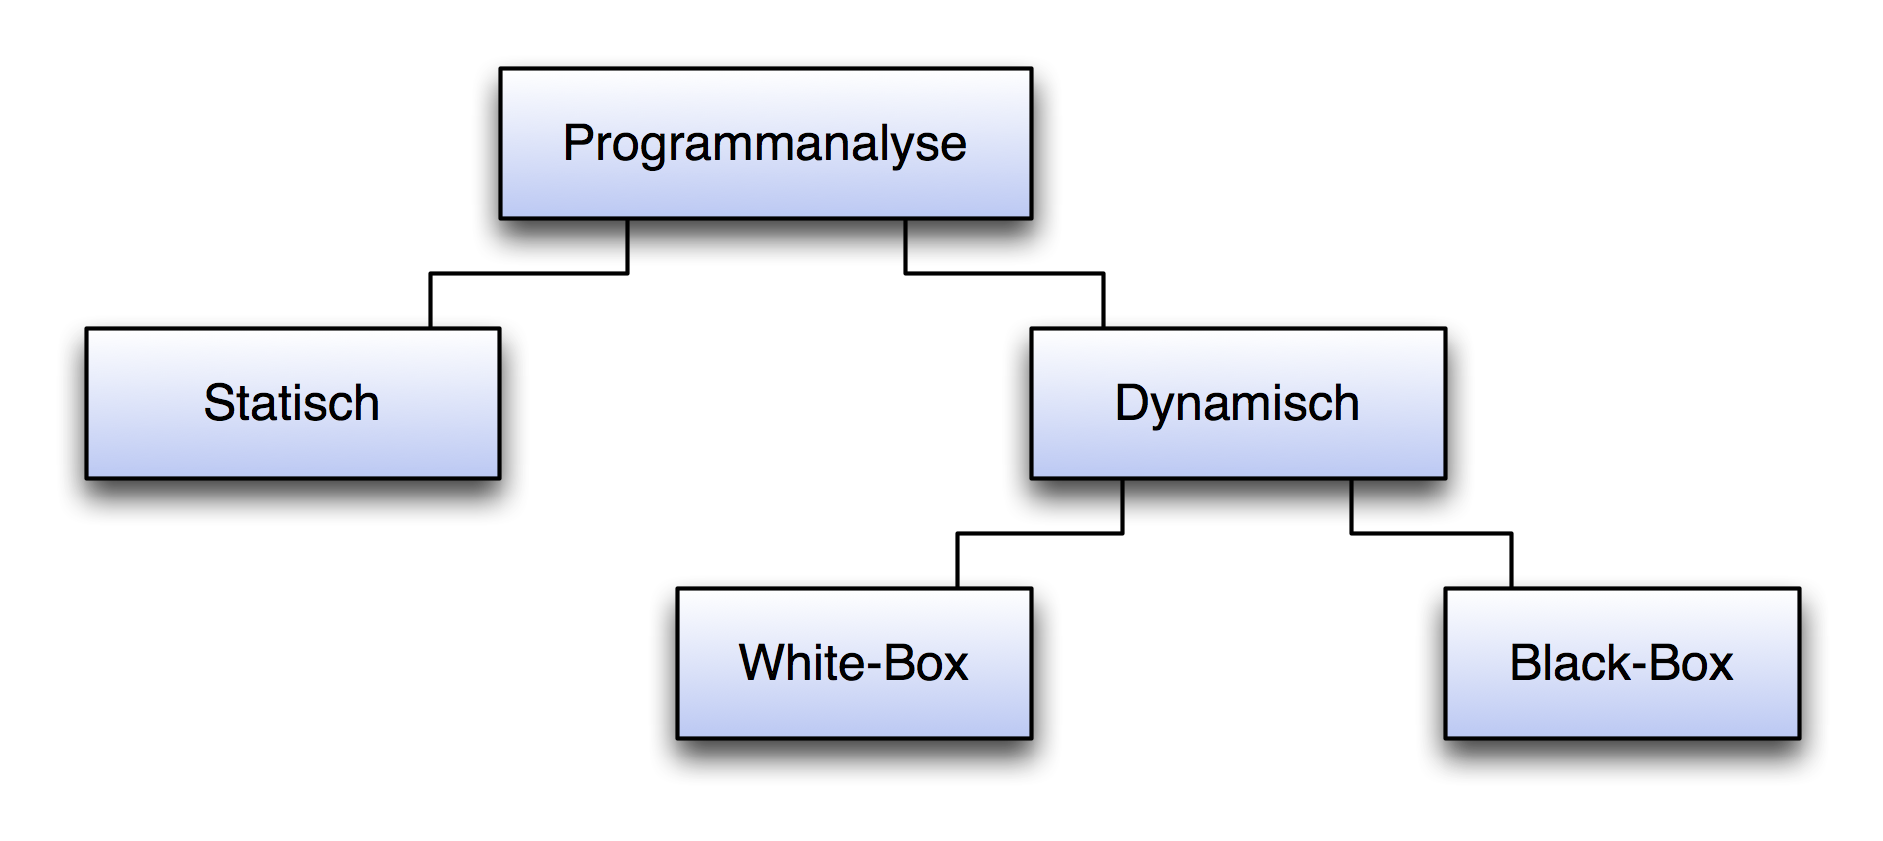
\includegraphics[width=0.6\textwidth]{./image/programmanalyse.png}
      \caption{Überblick über konventionelle Testmethoden (nach
      \cite{SoftwareanalyseBegriffeUndTechniken} S. 5)}
      \label{img:programmanalyse}
    \end{center}
  \end{figure}
  
  \subsection{Statische Programmanalyse}

  Die statische Programmanalyse basiert auf der Anaylse des Sourcecodes. Das
  bedingt, dass der Sourcecode zugägnglich ist. Als Softwareentwickler, kennt
  man das Verfahren eventuell aus der integrierten Entwicklungsumbegung
  (\acs{IDE})\acused{IDE}. Es gibt \acp{IDE}, wie zum Beispiel IntelliJ, siehe
  \cite{StaticCodeAnalysisIntelliJ}, die das Verfahren der statischen
  Programmanalyse nutzen. Wenn man Code schreibt, dann analysieren die
  \acp{IDE} den geschriebenen Code auf dessen syntaktische, semantische und
  lexikalische Informationen, siehe
  \cite{SoftwareQualitaetsmanagementInDerPraxis} S. 216f.
  
  Im Artikel \cite{GUIAnalysenUndBibliotheken} befasst sich der Author damit,
  was man bei \ac{GUI} lastiger Software durch eine statische Programmanaylse in
  Erfahrung bringen kann. Nach Aussage des Authors kann man bei deren
  Vorgeschlagenen Techniken folgendes erreichen:
  
  ``\begin{itshape}Im Rahmen dieser Analyse wird erkannt, welche Teile des
  Programms zur GUI gehören, welche Widgets das Programm enthält, welche
  Attribute, mit ihren Werten, diese Widgets besitzen, wie diese Widgets mit
  Events untereinander verbunden sind und wie sie in den einzelnen Fenstern der
  GUI strukturiert
  sind.\end{itshape}''\footnote{\cite{GUIAnalysenUndBibliotheken}
  Zusammenfassung - Seite 1}
    
  \subsection{Dynamische Programmanalyse}
  
  Bei der dynamischen Programmanalyse wir das zu analysierende Programm 
  ausgeführt. Die dynamische Programmanalyse wird in zwei Unterarten aufgeteilt,
  das Black-Box Verfahren und das White-Box Verfahren.
    
  \subsubsection{Black-Box Verfahren}
  
  Der Analyst hat keinerlei Informationen über das Innenleben des zu
  analysierenden Programms. Die Analyse basiert auf der intuitiven Bedienung der
  grafischen Oberfläche, durch den Analysten.
  
  \subsubsection{White-Box Verfahren}
  
  Der Analyst hat explizite Kenntnisse über das Innenleben des zu
  analysierenden Programms, zudem steht ihm der Sourcecode zur Verfügung. Mit
  der Hilfe des Sourcecodes können sinnvolle Schlüsse im Bezug auf die Analyse
  getroffen werden, da Spezialfälle, welche nicht offensichtlich sind,
  analysiert werden können. Als Beispiel dafür, möchte ich eine kurze
  Codesequenz zeigen, siehe Listing \ref{lst:dreifacherMausklick} Zeile 4.
  Dabei wird auf einen dreifachen Mausklick abgefragt. Da ein solches Verhalten nicht
  intuitiv ist, würde das ohne Sourcecode wahrscheinlich nicht gefunden werden.:
  \newline
  %\newpage
  
  \begin{lstlisting}[
    captionpos=b,
    caption=Spezialfall - dreifacher Mausklick,
    label=lst:dreifacherMausklick
  ]
  component.addMouseListener(new MouseAdapter() {
    public void mouseClicked(MouseEvent evt) {
      if (evt.getClickCount() == 3) {
        System.out.println("triple-click");
      }
    }
  });
  \end{lstlisting}
  
  \subsection{Probleme bei der Verwendung von Bibliotheken}
  
  Gemäss \cite{GUIAnalysenUndBibliotheken} S. 1f. besteht ebenfalls ein Problem
  bei der Verwendung von Bibliotheken. Die Grundproblematik besteht darin,
  dass eine Bibliothek eventuell ohne Zugriff auf deren Sourcecode verwendet
  wird. Damit wird das Verfahren der statischen Programmanalyse und der
  dynamischen White-Box Programmanalyse unmöglich.
  
  Falls eine statische Programmanalyse angestrebt wird, und der Sourcecode der
  verwendeten Bibliotheken vorhanden ist, kann sich das negativ auf die
  Präzision der Analyse auswirken. Denn es ist üblich, dass Bibliotheken
  meisst um ein Vielfaches grösser sind als das zu analysierende Programm. Der
  Aufwand wird durch die grössere Menge an Sourcecode zudem erhöht.
  
  \section{Wahl des Verfahrens}
  
  Die Wahl des Verfahrens der Analyse soll wie in der Abbildung
  \ref{img:guiAnalyse} durchgeführt werden. Leider wurde während der
  Durchführung der Diplomarbeit kein sinnvoll einsetzbares Werkzeug zur
  statischen Programmanalyse für Java Swing Applikationen gefunden. Somit wurde
  im Falle von vorhandenem Quellcode nur das dynamische White-Box Verfahren
  angewendet.
  
  % Falls es dabei zu einer statischen
  %Programmanalyse kommen sollte, soll die wenn mögliche mit der \ac{IDE}
  %IntelliJ durchgeführt werden.
  
  \begin{figure}[ht]
    \begin{center}
      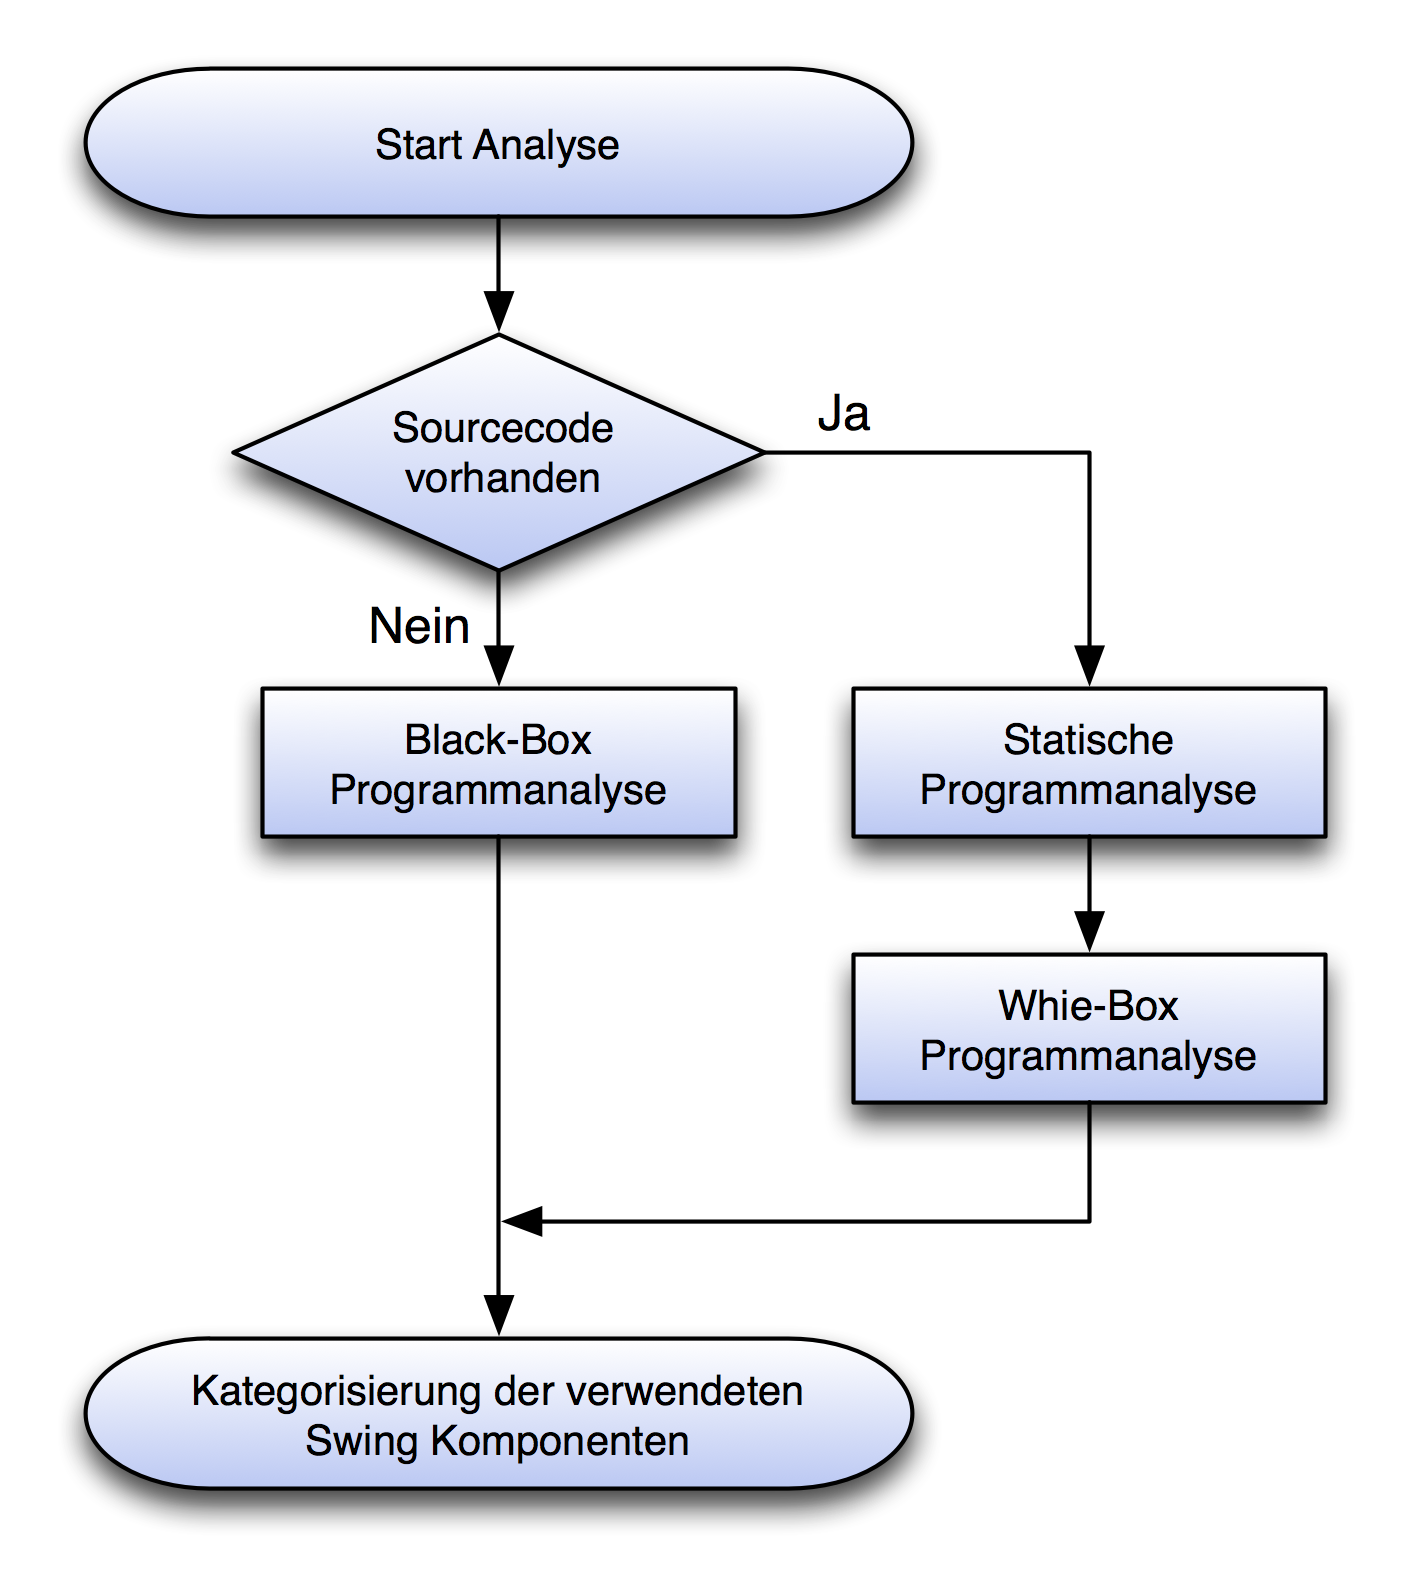
\includegraphics[width=0.5\textwidth]{./image/guiAnalyse.png}
      \caption{Wahl des Verfahrens der Programmanalyse}
      \label{img:guiAnalyse}
    \end{center}
  \end{figure}
  
  \section{Auswahl der Applikationen}
  
  Es sollen drei Applikationen, welche von der Zürcher Kantonalbank entwickelt
  wurden, analysiert werden. Die Applikationen sollen mit Java Swing entwickelt
  worden sein. Die Applikationen werden in der Tabelle
  \ref{tab:zuAnalysierendeJavaSwingApplikationen} aufgelistet.
  \newline
  
  \begin{table}[ht]
    \begin{center}
      \begin{tabular}{llr}
        \toprule
        Applikation & Version & Sourcecode vorhanden \\
        \midrule
        Strukti Live & Version 1.2 & Ja\\
        Strukti Online & Version 3.0 & Ja\\
        ?? & ?? & ??\\
        \bottomrule
      \end{tabular}
      \caption{Zu analysierende Java Swing Applikationen}
      \label{tab:zuAnalysierendeJavaSwingApplikationen}
    \end{center}
  \end{table}
  
  Strukti Live 1.2 wurde desshalb gewählt, weil es eine Applikation ist, die
  von der ZKB veröffentlicht wurde, somit werden bei der Anlayse keine
  sensiblen Informationen preisgegeben.
  
  Strukti Online 3.0 wurde desshalb gewählt, weil eine mögliche Migration zur
  Webapplikation schon einmal disskutiert wurde.
  
  \subsection{Strukti Live 1.2}
  
  Strukti Live ist ein Lerntool der Zürcher Kantonalbank für strukturierte
  Produkte. Die Applikation kann auf dem Internetauftritt der ZKB
  heruntergeladen werden. Unter der Internetadresse
  \url{http://www.zkb.ch/struktilive} sind alle nötigen Informationen
  enthalten.
  
  In der Tabelle \ref{tab:bibliothekenStruktiLive} sind alle verwendeten
  Bibliotheken, welche eine Interaktion mit dem \ac{GUI} haben, ersichtlich.
  \newline
  
  \begin{table}[ht]
    \begin{center}
      \begin{tabular}{lp{4.5cm}ccp{2cm}}
        \toprule
        Bibliothek & Funktion & Version & Lizenz & Quellcode vorhanden?\\
        \midrule
        core-renderer.jar & XHtml und CSS Renderer für Swing & R8 & LGPL & Ja\\
        %bogatyr\_0.60.jar & Abstraktion einiger Swing Komponenten & 0.60 & GPL
        %& Ja\\
        jfreechart-1.0.10.jar & Charting Library für Java & 1.0.10 & LGPL & Ja\\
        %jcommon-1.0.13.jar & JFreeChart extension & 1.0.13 & LGPL & Ja\\
        %ZKB\_CICD\_0.40.jar & Swing Komponenten im ZKB Design & 0.40 & - & Ja\\
        \bottomrule
      \end{tabular}
      \caption{Verwendete Bibliotheken von Strukti Live 1.2}
      \label{tab:bibliothekenStruktiLive}
    \end{center}
  \end{table}
  
  Gemäss der dynamischen White-Box Programmanalyse werden alle Komponenten, die
  Java Swing zur Verfügung stellt in der Applikation gesucht. Die Komponenten
  können in der Dokumentation zu Java Swing von Oracle gefunden werden, siehe
  \cite{SwingComponentsByOracle}. Zudem sollen alle Komponenten, welche durch
  externe Bibliotheken zur Verfügung gestellt werden, gesucht werden. Die
  Suche findet durch einen visuellen Vergleich der Komponenten statt, wenn
  nötig kann auch der Sourcecode in die Suche miteinbezogen werden. Es soll eine
  Auflistung aller gefundenen Komponenten erstellt werden.
  
  \subsubsection{Top-Level-Komponenten}
  
  \begin{itemize}
    \item \(javax.swing.JFrame\) mit javax.swing.JRootPane, siehe Abbildung
    \ref{img:SL-01}
    \item \(javax.swing.JDialog\), siehe Abbildung \ref{img:SL-02}
  \end{itemize}
  
  \subsubsection{Intermediate-Komponenten}
  
  \begin{itemize}
    \item \(javax.swing.JPanel\), siehe Abbildung \ref{img:SL-01}
    \item \(javax.swing.JScrollPane\), siehe Abbildung \ref{img:SL-01}
    \item \(javax.swing.JTabbedPane\), siehe Abbildung \ref{img:SL-03}
  \end{itemize}
  
  \subsubsection{Atomic-Komponenten}
  
  \begin{itemize}
    \item \(javax.swing.JLabel\), siehe Abbildung \ref{img:SL-01}
    \item \(javax.swing.JButton\), siehe Abbildung \ref{img:SL-01}
    \item \(javax.swing.JCheckBox\), siehe Abbildung \ref{img:SL-01}
    \item \(javax.swing.JSlider\), siehe Abbildung \ref{img:SL-02}
    \item \(javax.swing.JTextField\), siehe Abbildung \ref{img:SL-02}
    \item \(javax.swing.JRadioButton\), siehe Abbildung \ref{img:SL-02}
    \item \(javax.swing.JToolTip\), siehe Abbildung \ref{img:SL-03}
  \end{itemize}
  
  \subsubsection{Spezielle Komponenten}
  
  \begin{itemize}
    \item \(org.jfree.chart.JFreeChart\), siehe Abbildung \ref{img:SL-02}
    \item \(org.xhtmlrenderer.simple.XHTMLPanel\), siehe Abbildung
    \ref{img:SL-03}
    \item \(javax.swing.JLabel\) als externer Link, siehe Abbildung
    \ref{img:SL-03}
  \end{itemize}
  
  \begin{figure}[htb]
    \begin{center}
      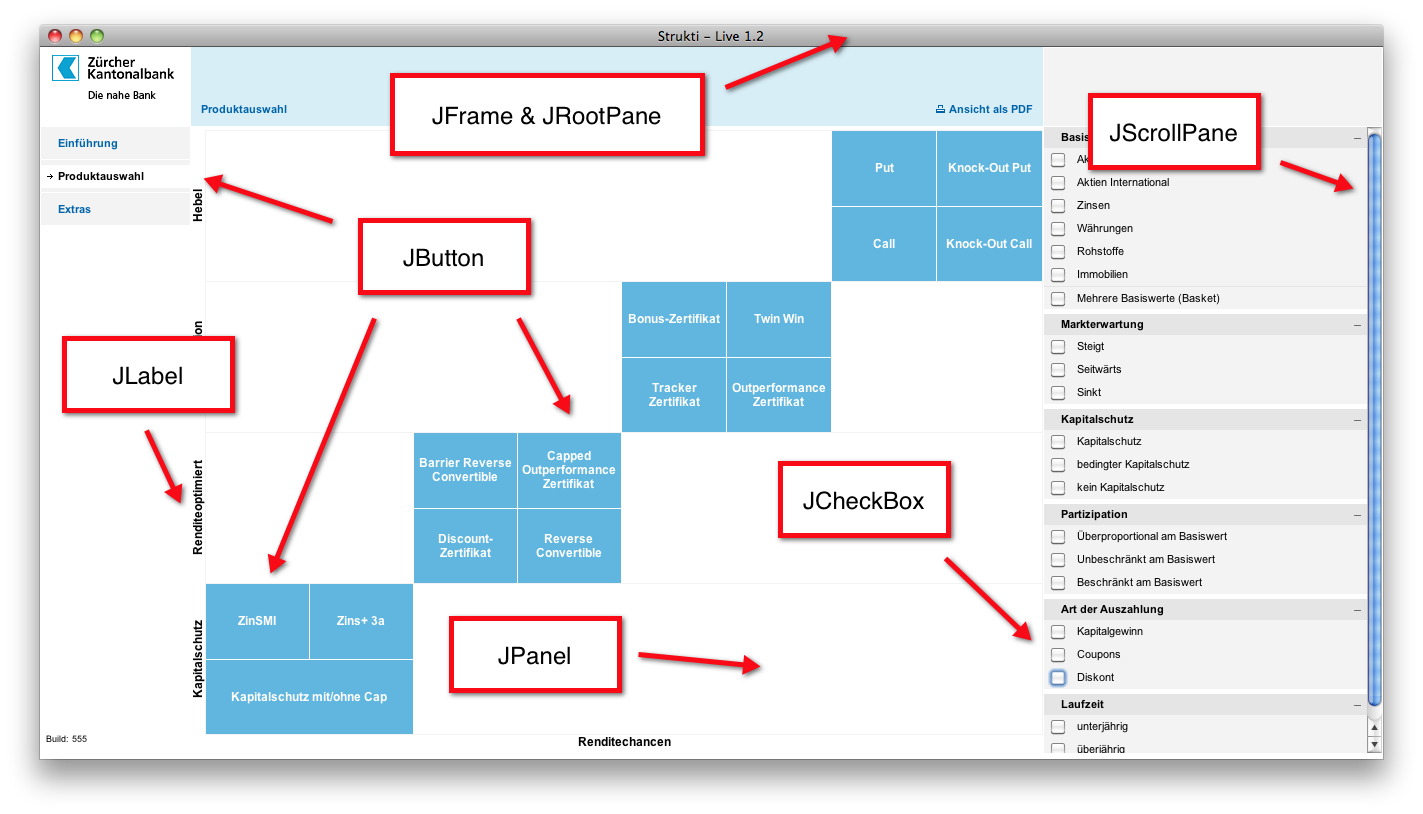
\includegraphics[width=\textwidth]{./image/SL/SL-01.png}
      \caption{Strukti Live 1.2 - Screenshot I}
      \label{img:SL-01}
    \end{center}
  \end{figure}
  
  \begin{figure}[htb]
    \begin{center}
      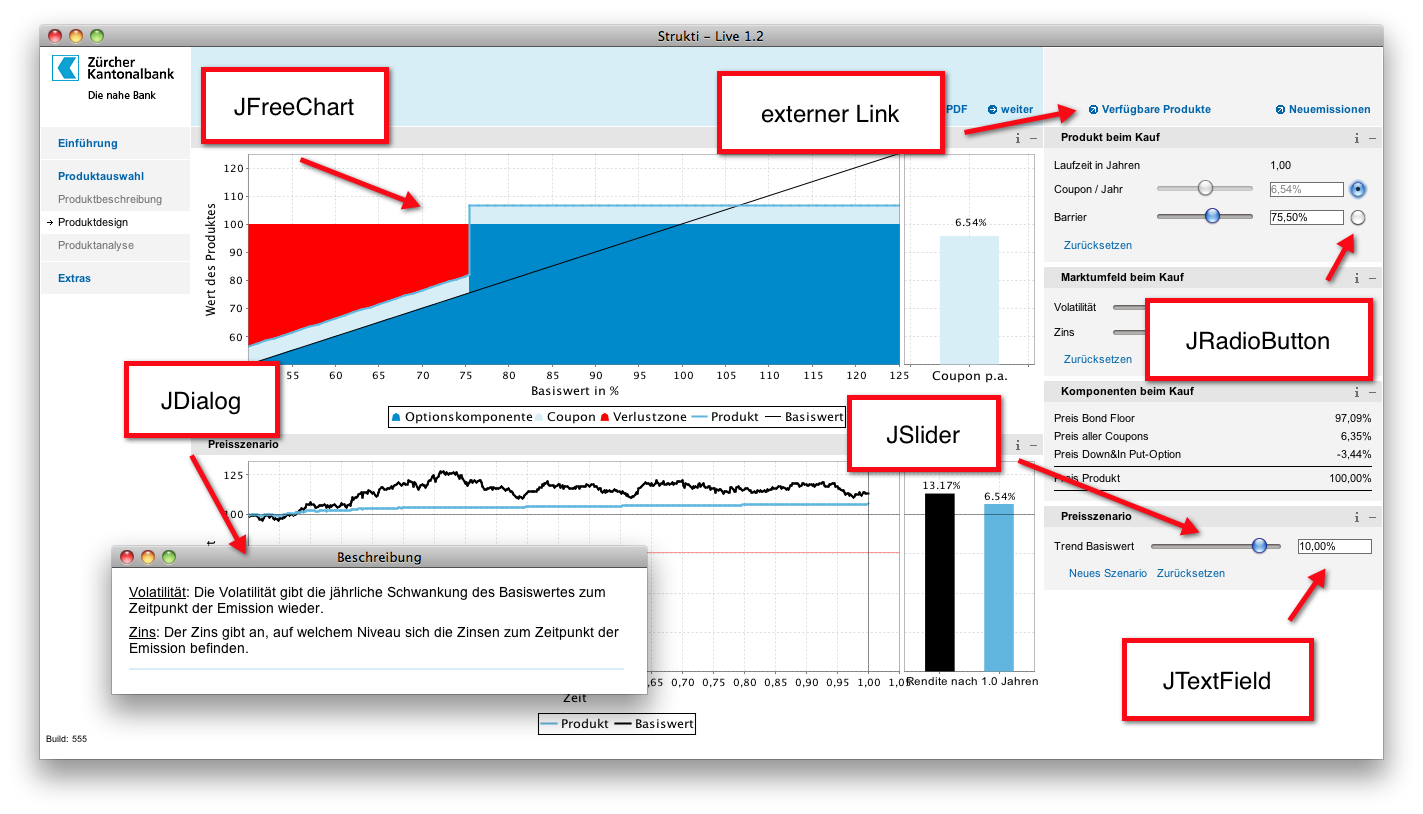
\includegraphics[width=\textwidth]{./image/SL/SL-02.png}
      \caption{Strukti Live 1.2 - Screenshot II}
      \label{img:SL-02}
    \end{center}
  \end{figure}
  
  \begin{figure}[htb]
    \begin{center}
      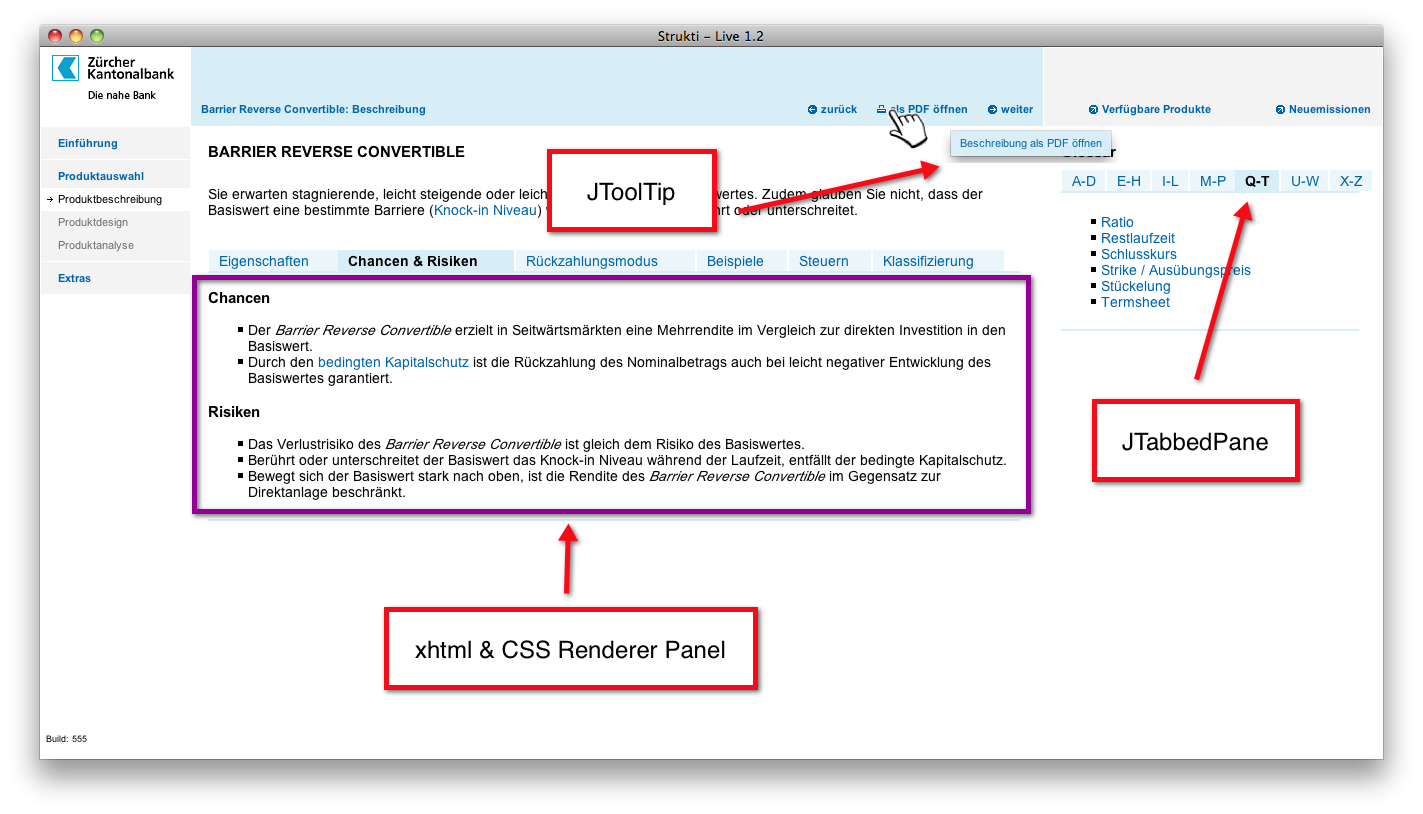
\includegraphics[width=\textwidth]{./image/SL/SL-03.png}
      \caption{Strukti Live 1.2 - Screenshot III}
      \label{img:SL-03}
    \end{center}
  \end{figure}
  
  \subsubsection{Zusammenspiel von Komponenten}

  Durch das Zusammenspiel einzelner Komponenten können ``neue'' Komponenten
  entstehen. In Strukti Live wurden folgende erkannt und mit einem
  entsprechenden Namen versehen.
  
  \begin{description}
    \item[Button-Matrix]
    Buttons werden in einer Matrix angeordnet, um sie entsprechend ihrer
    Funktion zu ordnen. Dabei können die Buttons entsprechend ihrer
    Renditechancen (x-Achse) und deren Kapitalschutz (y-Achse) eingeordnet
    werden.
    \item[Akkordeon]
    Ein Verbund von \(javax.swing.JPanel\) Komponenten, bei welchem ein
    Panel als Titelleiste funktioniert. In der Titelleiste kann über ein Minus-
    oder Plussymbol ein weiterer Panel ein- oder ausgeklappt werden.
    \item[Filter]
    Es wurde ein Filter mit \(javax.swing.JCheckBox\) Komponenten implementiert.
    Die möglichen Filteroptionen werden als Checkbox dargestellt und können
    somit aus- beziehungsweise eingeschalten werden.
    \item[Menüführung]
    Die Menüführung wurde durch das Observer-Pattern, siehe
    \cite{ObserverEntwurfsmuster}, implementiert. Dabei wird in einem Modell
    der jeweilige Status der Applikation durch das Drücken eines
    \(javax.swing.JButton\) angepasst, wobei sich die jeweiligen
    \(javax.swing.JPanel\), welche auf Änderungen des Modells höhren, sich neu
    zeichnen.
    \item[Komponentenupdate]
    Ebenfalls mit dem Observer-Pattern, siehe \cite{ObserverEntwurfsmuster},
    wurde die Aktualisierung von Komponenten, welche zusammen hängen,
    realisiert. Als Beispiel dient ein Verbund der Komponenten
    \(javax.swing.JTextField\), \(javax.swing.JSlider\) und
    \(org.jfree.chart.JFreeChart\). Dabei werden bei einer Änderung des Wert bei
    dem Slider oder dem Textfeld alle anderen Komponenten entsprechend
    aktualisiert.
  \end{description}
  
  \subsection{Strukti Online 3.0}
  
  Strukti Online ist ein Emissionstool der Zürcher Kantonalbank für
  strukturierte Produkte. Die Applikation wird aktuell nur zum internen
  Gebrauch entwickelt.
  
  In der Tabelle \ref{tab:bibliothekenStruktiOnline} sind alle verwendeten
  Bibliotheken, welche eine Interaktion mit dem \ac{GUI} haben, ersichtlich,
  und ob deren Sourcecode zugänglich ist.
  
  \begin{table}[ht]
    \begin{center}
      \begin{tabular}{lllr}
        \toprule
        Bibliothek & Version & Lizenz & Sourcecode vorhanden \\
        \midrule
        Swingx & xx & xx & Ja\\
        JFreeChart & xx & xx & Ja\\
        \bottomrule
      \end{tabular}
      \caption{Verwendete Bibliotheken von Strukti Online X.X}
      \label{tab:bibliothekenStruktiOnline}
    \end{center}
  \end{table}
  
  \section{Kategorisierung von verwendeten Swing Komponenten}